\documentclass[12pt]{article}
\usepackage[utf8]{vietnam}
%\usepackage[english]{babel}
\usepackage[T5]{fontenc}
\usepackage[top=2cm, bottom=2cm, left=2cm,right=2cm]{geometry} %%%% Margin %%%%%
\usepackage[dvipsnames]{xcolor}
\usepackage[pdftex]{graphicx}
\usepackage{wrapfig}
\usepackage{tcolorbox}
\usepackage{mathtools}
\usepackage{amsmath}
\usepackage{amssymb}
\usepackage{eqnarray}
\usepackage{siunitx}
\usepackage{array, lipsum, bibentry,fancyhdr}
\usepackage{hyperref}
\usepackage{natbib}
\setlength{\parindent}{0pt}
\usepackage{enumitem}
\usepackage[noframe]{showframe}
\usepackage{framed}
\usepackage{titling}
\usepackage{float}
\usepackage{multicol}
\usepackage{url}
\usepackage{authblk}
\usepackage{sectsty}
\usepackage{eqparbox}

%%%%%%%%%% Pictures drawing %%%%%%%%%%%%%

\usepackage{pgfplots} %%%%%% Regression %%%%
\pgfplotsset{compat = newest}
\usepackage{pgfplotstable}
\usepackage{tikz}
\usepackage{tikz-3dplot} %%%%%% Draw %%%%%%
\usepackage{tikz,tkz-euclide}
\usetikzlibrary{arrows,calc,patterns}
\usetikzlibrary{quotes,angles}
\usetikzlibrary{shapes.geometric}
\usepackage{circuitikz} %%%%% Circuit %%%%
\usetikzlibrary{decorations.pathmorphing,patterns}

\setlength{\unitlength}{1cm}

%%%%%%%%%% Hyperlink %%%%%%%%%%%%%

\hypersetup{
	colorlinks=true,
	linkcolor=black,
	filecolor=mangeta,      
	urlcolor=blue,
	pdftitle={Overleaf Example},
	pdfpagemode=FullScreen,
}

%%%%%%%%%% Header & Footer %%%%%%%%%%%%%

\setlength{\headheight}{10mm}
\RequirePackage{fancyhdr}  % Needed to define custom headers/footers
\RequirePackage{lastpage}  % Number of pages in the document
\pagestyle{fancy}          % Enables the custom headers/footers
% Headers
%\lhead{\includegraphics[width=.8in]{xPhO.png}}%
\chead{}%
\rhead{\small\sffamily\bfseries{Phương pháp giải các bài toán dao động} --- \thepage/\pageref{LastPage}}
% Footers
\lfoot{}%
\cfoot{}%
\rfoot{}%
\renewcommand{\headrulewidth}{1pt}% % header rule
\renewcommand{\footrulewidth}{1pt}% % footer rule

% \pagestyle{fancy}
% 	\fancyhead[L]{\empty}
% 	\fancyhead[R]{\empty}
% 	\fancyhead[C]{\empty}
% 	\fancyfoot[C]{\empty}
% 	\fancyfoot[L]{\empty}
% 	\renewcommand{\headrulewidth}{0pt}
% 	\fancyfoot[C]{\normalcolor{\thepage/\pageref{LastPage}}}
% 	\setcounter{page}{1}

%%%%%%%%%% Color setup %%%%%%%%%%%%%

\RequirePackage{xcolor}
\definecolor{wsdred}{HTML}{8E1728}
\definecolor{wsdgrey}{HTML}{75787B}
\renewcommand{\normalcolor}{\color{wsdred}}
\colorlet{ColorOr}{white}

\begin{document}

%% Title %%
{\fontsize{50}{24}\fontfamily{phv}\fontseries{b}
\LARGE \normalcolor{ \textbf{Dao động cơ học} } }

\textcolor{blue}{\textbf{\textit{Câu lạc bộ vật lý xPhO}}}
\vspace{3mm}

Trong phần này, chúng ta sẽ tìm hiểu về chuyển động dao động. Bắt đầu từ những thứ cơ bản nhất như con lắc đơn, đến những hệ phức tạp như dao động liên kết giữa các vật. 

\tableofcontents
\newpage


\section{Dao động hệ 1 chất điểm}
\subsection{Dao động điều hoà}
Đầu tiên chúng ta xem xét hệ cơ bản nhất của dao động. Chỉ bao gồm duy nhất 1 chất điểm có khối lượng \(m\). Trong quá trình chuyển động của chất điểm, nó phải chịu một lực có dạng \(F = - k x\). Lực này có đặc điểm luôn hướng về vị trí có \(x = 0\). 

\begin{figure}[!htb]
    \centering
    \input{Image/1.1}
    \caption{}
    \label{fig:1.1}
\end{figure}

Ta sẽ dễ dàng viết được phương trình vi phân chuyển động (Hay nói cách khác chính là phương trình định luật II Newton).
\begin{equation}
    m \ddot{x} = -kx.
    \label{eq:1.1}
\end{equation}
Từ các phương pháp giải phương trình vi phân, ta có thể thu được nghiệm của phương trình trên.
\begin{equation}
    x = A \cos{ \left(\omega t + \varphi \right)}.
    \label{eq:1.2}
\end{equation}
Với \(A\) là biên độ; \(\omega = \sqrt{k/m}\) là tần số góc; \(\varphi\) góc thể hiện vị trí ban đầu. 
\vspace{4mm}

Ta có nhiều cách để biểu diễn một phương trình dao động tương tự như phương trình \ref{eq:1.2}. Ta có thể biểu diễn phương trình dao động bằng số phức.
\begin{equation}
    x^* = A e^{i \left( \omega t + \varphi \right)}.
    \label{eq:1.2-2}
\end{equation}
Cách này không làm thay đổi tính đúng đắn của phương trình dao động và hoàn toàn tương đương phương trình \ref{eq:1.2}. Để giải thích, ta sử dụng công thức Euler.
\begin{equation*}
    x^* = A \cos{\left( \omega t + \varphi \right)} + i A \sin{\left( \omega t + \varphi \right)}.
\end{equation*}
Ta thấy rằng phương trình \ref{eq:1.2} là phần thực của phương trình \ref{eq:1.2-2}. Ta có liên hệ
\begin{equation}
    x = Re (x^*).
\end{equation}
\subsection{Dao động có cản}
Ở hệ dao động trên, chỉ có lực dạng lực lò xo tác dụng lên vật. Vật sẽ chuyển động điều hoà vĩnh viễn. Nhưng trong thực tế, luôn tồn tại những lực ma sát làm suy giảm chuyển động của hệ. 


\subsubsection{Lực ma sát khô (ma sát trượt)}

Lực ma sát khô (hay ma sát trượt) là lực có dạng sau. Lực này có đặc điểm luôn ngược chiều với xu hướng chuyển động của hệ vật. Hay nói chính xác hơn là lực này ngược chiều với chiều vận tốc hệ vật. Độ lớn của lực thường là hằng số trong các trường hợp cơ bản.

\begin{equation}
\begin{array}{ccc}
    F_1 = - \mu N &\text{Hoặc} & \Vec{F_1} = - \mu N {\displaystyle  \frac{\Vec{v}}{|\Vec{v}|}}. \\
    \text{Với} \ N = mg & &
\end{array}
\label{eq:1.3}
\end{equation}

\begin{figure}[!htb]
    \centering
    \scalebox{0.8}{\input{Image/1.2}}
    \caption{}
    \label{fig:1.2}
\end{figure}


Ta thấy rằng, hướng của lực ma sát bị thay đổi trong quá trình chuyển động. Một cách tổng quát, ta có thể sử dụng dạng vector của lực ma sát. Nhưng như thế thì khá khó để giải quyết. Ta sẽ chia thành 2 quá trình, quá trình (1) là khi vật đang đi theo chiều dương; quá trình (2) là khi vật đang đi theo chiều âm.



\vspace{2mm}

\underline{\textit{Quá trình (1): chuyển động theo chiều dương.}}
\vspace{2mm}

Khi này, lực ma sát sẽ luôn hướng theo chiều âm trong cả quá trình. Ta viết được phương trình vi phân chuyển động
\begin{equation}
    m \ddot{x} =  - k x - \mu  m g.
    \label{eq:1.4}
\end{equation}
Để giải phương trình vi phân này, ta sẽ đặt biến là $u = x + \mu mg/k$. Thực hiện việc đổi biến, ta thu được phương trình
\begin{equation*}
    \ddot{u} + {\frac{k}{m} \displaystyle} u = 0.
\end{equation*}
Từ đó ta thu được nghiệm có dạng
\begin{equation}
    \begin{split}
        u &= A_n \cos{\left(\sqrt{k/m} \ t + \varphi \right)} \\
        \Rightarrow x &= A_n \cos{\left(\sqrt{k/m} \ t + \varphi \right)} - {\displaystyle \frac{\mu m g}{k}}.
    \end{split}
    \label{eq:1.5}
\end{equation}
Phương trình này giống hệ như một phương trình dao động điều hoà. Nhưng vị trí cân bằng bị lệch đi một đoạn $OO' = \mu m g/k$, $O'$ là vị trí cân bằng mới. Điểm $O'$ bị lệch về phía chiều âm so với $O$.
\begin{figure}[!htb]
    \centering
    \input{Image/1.3}
    \caption{}
    \label{fig:1.3}
\end{figure}

Ta sẽ suy ra được một số điều sau
\begin{enumerate}
    \item \(O'A_0 = O'A_1 = \alpha\).
    \item 
    \(
    \left\{
        \begin{array}{ccc}
        OA_0 &=& \alpha + \mu mg/k. \\ 
        OA_1 &=& \alpha - \mu mg/k.
        \end{array}
    \right.
    \)
    
    Hay sau mỗi \(T/2\) thì biên độ mới và cũ sẽ có sự chênh lệch
    \(OA_1 = OA_0 - 2 \mu mg/k\).
\end{enumerate}
\vspace{2mm}

\underline{\textit{Quá trình (2): chuyển động theo chiều âm.}}
\vspace{2mm}

Khi này, lực ma sát sẽ luôn hướng theo chiều âm trong cả quá trình. Ta viết được phương trình vi phân chuyển động
\begin{equation}
    m \ddot{x} =  - kx + \mu m g.
    \label{eq:1.6}
\end{equation}
Tương tự với quá trình (1), ta đặt biến là $v = x - \mu mg/k$. Ta thu được phương trình
\begin{equation*}
    \ddot{v} + {\frac{k}{m} \displaystyle} v = 0.
\end{equation*}
Từ đó ta thu được nghiệm có dạng
\begin{equation}
    \begin{split}
        v &= B_n \cos{\left(\sqrt{k/m} \ t + \varphi \right)} \\
        \Rightarrow x &=  B_n \cos{\left(\sqrt{k/m} \ t + \varphi \right)} + {\displaystyle \frac{\mu m g}{k}}.
    \end{split}
    \label{eq:1.7}
\end{equation}

Phương trình này cũng tương tự như phương trình dao động. Nhưng ở trường hợp này thì vị trí cân bằng bị lệch về phía chiều dương so với $O$, $OO' = \mu mg/k$. 

\begin{figure}[!htb]
    \centering
    \input{Image/1.4}
    \caption{}
    \label{fig:1.4}
\end{figure}

Ta sẽ suy ra được một số điều sau
\begin{enumerate}
    \item \(O'A_0 = O'A_1 = A\).
    \item 
    \(
    \left\{
        \begin{array}{ccc}
        OA_0 &=& A + \mu mg/k. \\ 
        OA_1 &=& A - \mu mg/k.
        \end{array}
    \right.
    \) 

    Hay sau mỗi \(T/2\) thì biên độ mỡi và cũ sẽ có sự chênh lệch
    \(OA_1 = OA_0 - 2 \mu mg/k\).
\end{enumerate}

**Lý do tại sao phải ghi rõ là biên độ thứ n, bởi vì biên độ của vật sẽ giảm dần và khác nhau biệt lẫn nhau. Biên độ sẽ bị thay đổi ở mỗi "nửa" chu kỳ. 
\vspace{2mm}

\underline{\textit{Ví dụ trực quan}}

Chúng ta sẽ xét một ví dụ đơn giản (hình \ref{fig:1.5}) để có thể hiểu tốt phần này. Ta thả một vật cách vị trí lò xo đang co và cách vị trí không giãn một đoạn $A_0$.
\vspace{2mm}

\begin{enumerate}[label = \textbullet]
    \item Khi từ trạng thái (A) sang trạng thái (B). Thì biên độ của vật giảm \(2\mu mg/k \). \\ Hay \(A_0 - A_1 = 2 \mu mg/k\). Quá trình này tốn nửa chu kỳ.
    \item Khi đi từ trạng thái (B) sang trạng thái (C). Thì biên độ của vật cũng giảm \(2\mu mg/k \). \\ Hay \(A_1 - A_2 = 2 \mu mg/k\). Quá trình này tốn nửa chu kỳ.
\end{enumerate}




\begin{figure}[!htb]
    \centering
    \scalebox{0.8}{\input{Image/1.5}}
    \caption{}
    \label{fig:1.5}
\end{figure}

Vậy thì ta có công thức liên hệ giữa các biên độ liền kề nhau.

\begin{equation}
    A_{k+1} = A_{k} - 2 \mu mg/k.
\end{equation}


\subsubsection{Lực ma sát nhớt}

\begin{figure}[!htb]
    \centering
    \input{Image/1.6}
    \caption{}
    \label{fig:1.6}
\end{figure}

Lực ma sát nhớt sẽ bị phụ vào độ lớn và hướng của vận tốc hệ vật theo biểu thức sau. Ở đây lực ma sát nhớt mà chúng ta khảo sát là lực phụ thuộc bậc 1 vào vận tốc hệ vật\footnote{Tồn tại lực ma sát nhớt phụ thuộc bậc 2 vào vận tốc vật. Nhưng trong bài toán này ta không xét tới.}. 
\begin{equation}
    \vec{F}_2 = - b \vec{v}.
    \label{eq:1.8}
\end{equation}
Ta có thể viết được phương trình vi phân chuyển động của nó.
\begin{equation*}
    m \ddot{x} = - k x - b \dot{x}.
\end{equation*}
Đây chính là phương trình vi phân bậc 2, để trở thành đúng dạng đã học thì ta sẽ ghi thành
\begin{equation}
    \ddot{x} + {\displaystyle \frac{b}{m}} \dot{x} + {\displaystyle \frac{k}{m}} x = 0. 
    \label{eq:1.9}
\end{equation}
Ta giả sử \(x = A e^{\lambda t}\). Thay nó vào phương trình \ref{eq:1.9}. Ta đặt \(b/m = 2 \gamma\), \(\omega = \sqrt{k/m}\).
\begin{equation*}
    \lambda^2 + (2\gamma) \lambda + \omega^2 = 0.
\end{equation*}

Tính \(\Delta\) của phương trình bậc 2, ta thu được
\begin{equation}
    \Delta = 4 \gamma^2 - 4 \omega^2
    \label{eq:1.10}
\end{equation}
\vspace{2mm}

\underline{\textit{Trường hợp (1): $\Delta$ < 0 - Lực cản nhỏ}}

Ta thu được \(\lambda\) và nghiệm tổng quát của phương trình vi phân.
\begin{equation}
    \left\{
    \begin{array}{ccc}
    \lambda &=& - \gamma \pm  i \sqrt{\omega^2 - \gamma^2} \\
    x &=& e^{-\gamma t} \left(A e^{i\sqrt{\omega^2 - \gamma^2} \ t} + B e^{- i\sqrt{\omega^2 - \gamma^2} \ t} \right).
    \end{array}
    \right.
\end{equation}

Nhưng kết quả ta thu được buộc phải là số thực, vậy nên các hằng số $A, B$ sẽ đảm bảo cho $x$ là một số thực. Cụ thể thì $A$ và $B$ phải có liên hệ
\begin{equation*}
    \left\{
    \begin{array}{ccc}
    A + B &=& C \cos \phi \\
    A - B &=& i C \sin \phi
    \end{array}
    \right.
\end{equation*}
Vậy thì ta sẽ thu được nghiệm tổng quát \(x\) như sau
\begin{equation}
\begin{split}
    x = \equiv e^{-\gamma t} C \cos{\left(\sqrt{\omega^2 - \gamma^2} \ t + \phi \right)}
\end{split}
\end{equation}

\begin{figure}[!htb]
    \centering
    \begin{tikzpicture}[scale=1]
      \begin{axis}[
          domain=0:5,
          samples=100,
          axis lines=middle,
          xlabel=$t$,
          ylabel=$x$
        ]
        \addplot[blue, thick, dash pattern=on 5pt off 2pt] {e^(-x)};
        \addplot[blue, thick, dash pattern=on 5pt off 2pt] {-e^(-x)};
        \addplot[blue, thick] {e^(-x)*cos(deg(5*x + 5))};
      \end{axis}
    \end{tikzpicture}
    \caption{Hàm \(e^{-t} \cos{\left(5t + 5 \right)}\)}
    \label{fig:1.7}
\end{figure}

\newpage
\vspace{2mm}

\underline{\textit{Trường hợp (2): \(\Delta\) > 0 - Lực cản lớn}}

Ta thu được \(\lambda\) và nghiệm tổng quát của phương trình vi phân.
\begin{equation}
    \left\{
    \begin{array}{ccc}
    \lambda &=& - \gamma \pm   \sqrt{\gamma^2 - \omega^2} \\
    x &=& A e^{- \left( \gamma - \sqrt{\gamma^2 - \omega^2}\right)  t} + B e^{- \left( \gamma + \sqrt{\gamma^2 - \omega^2}\right) t}.
    \end{array}
    \right.
\end{equation}

Trong trường hợp lực cản lớn, vật sẽ không thực hiện quá trình dao động. Mà bị tắt dần (nhưng chậm).

\begin{figure}[!htb]
    \centering
    \begin{tikzpicture}[scale=1]
      \begin{axis}[
          domain=0:2,
          samples=100,
          axis lines=middle,
          xlabel=$t$,
          ylabel=$x$
        ]
        \addplot[blue, thick] {20*e^(-(5-2)*x) +10*e^(-(5+2)*x};
      \end{axis}
    \end{tikzpicture}
    \caption{Hàm \(20 e^{-(5-2)t} + 10 e^{-(5+2)t}\)}
    \label{fig:1.8}
\end{figure}
\vspace{2mm}

\underline{\textit{Trường hợp (3): \(\Delta = 0\) - Tới hạn}}

Trong trường hợp này, khi ta giải phương trình bậc 2 nó sẽ bị trùng nghiệm. Và ta sẽ không thể áp dụng cách đã làm với trường hợp (1) và (2) vào đây được. Lúc này, dựa vào lý thuyết để giải phương trình vi phân, ta sẽ biết dạng tổng quát của \(x\).Chuyển động sẽ tắt dần rất nhanh. 
\begin{equation}
    \left\{
    \begin{array}{ccc}
    \lambda &=& \omega = \gamma \\
    x &=& e^{-\gamma t} \left( A + B t\right).
    \end{array}
    \right.
\end{equation}

\begin{figure}[!htb]
    \centering
    \begin{tikzpicture}[scale=1]
      \begin{axis}[
          domain=0:2,
          samples=100,
          axis lines=middle,
          xlabel=$t$,
          ylabel=$x$
        ]
        \addplot[blue, thick] {e^(-5*x)*(20 + 10*x)};
      \end{axis}
    \end{tikzpicture}
    \caption{Hàm \(e^{-5t} \left(20 + 10t\right)\)}
    \label{fig:1.9}
\end{figure}
\vspace{2mm}

Tóm lại, với trường hợp có lực cản nhớt trong hệ thì ta có một vài trường hợp xảy ra. Từ đấy, ta tổng hợp thành một bảng. Xét phương trình đặc trưng của phương trình vi phân bậc 2 là:
\begin{equation*}
    a\lambda^2 + b\lambda + c = 0
\end{equation*}

\begin{table}[!htb]
    \centering
    \begin{tabular}{| >{\centering\arraybackslash}m{5cm} | >{\centering\arraybackslash}m{8cm} |}
    \hline
    Phương trình bậc 2 của \(\lambda\) & Dạng nghiệm \\
    \hline
    Vô nghiệm &\rule{0pt}{0.7cm} 
    \(x = C \exp{\left(- \frac{b}{2a} \displaystyle \right)} \cos{\left(\sqrt{4 ac - b^2} \ t + \phi \right)} \).
    \\
    \hline
    2 nghiệm phân biệt & \(6\)
    
    \end{tabular}
    \caption{Caption}
    \label{tab:my_label}
\end{table}

\subsection{Dao động có lực cưỡng bức}
Khi này, hệ vật chịu thêm một lực từ một nguồn khác. Lực này có dạng là một dạng lực điều hoà.
\begin{equation}
    F(t) = F_0 \cos{\left(\Omega t + \phi \right)}.
\end{equation}
Lực này cưỡng bức vật và khiến cho chuyển động theo có xu hướng theo chu kỳ của lực cưỡng bức. Ta viết phương trình vi phân chuyển động của hệ.
\begin{equation}
    m \ddot{x} + b \dot{x} + k x= F_0 \cos{\left(\Omega t + \phi \right)}.
\end{equation}

\end{document}
